\Chapter{}{Software documentation}\label{apx:doc}
Going from general picture to details the program is designed to be started by running main.vi (which is happening upon boot or can be done manually whenever desired).
\begin{figure}[!h]
    \centering
    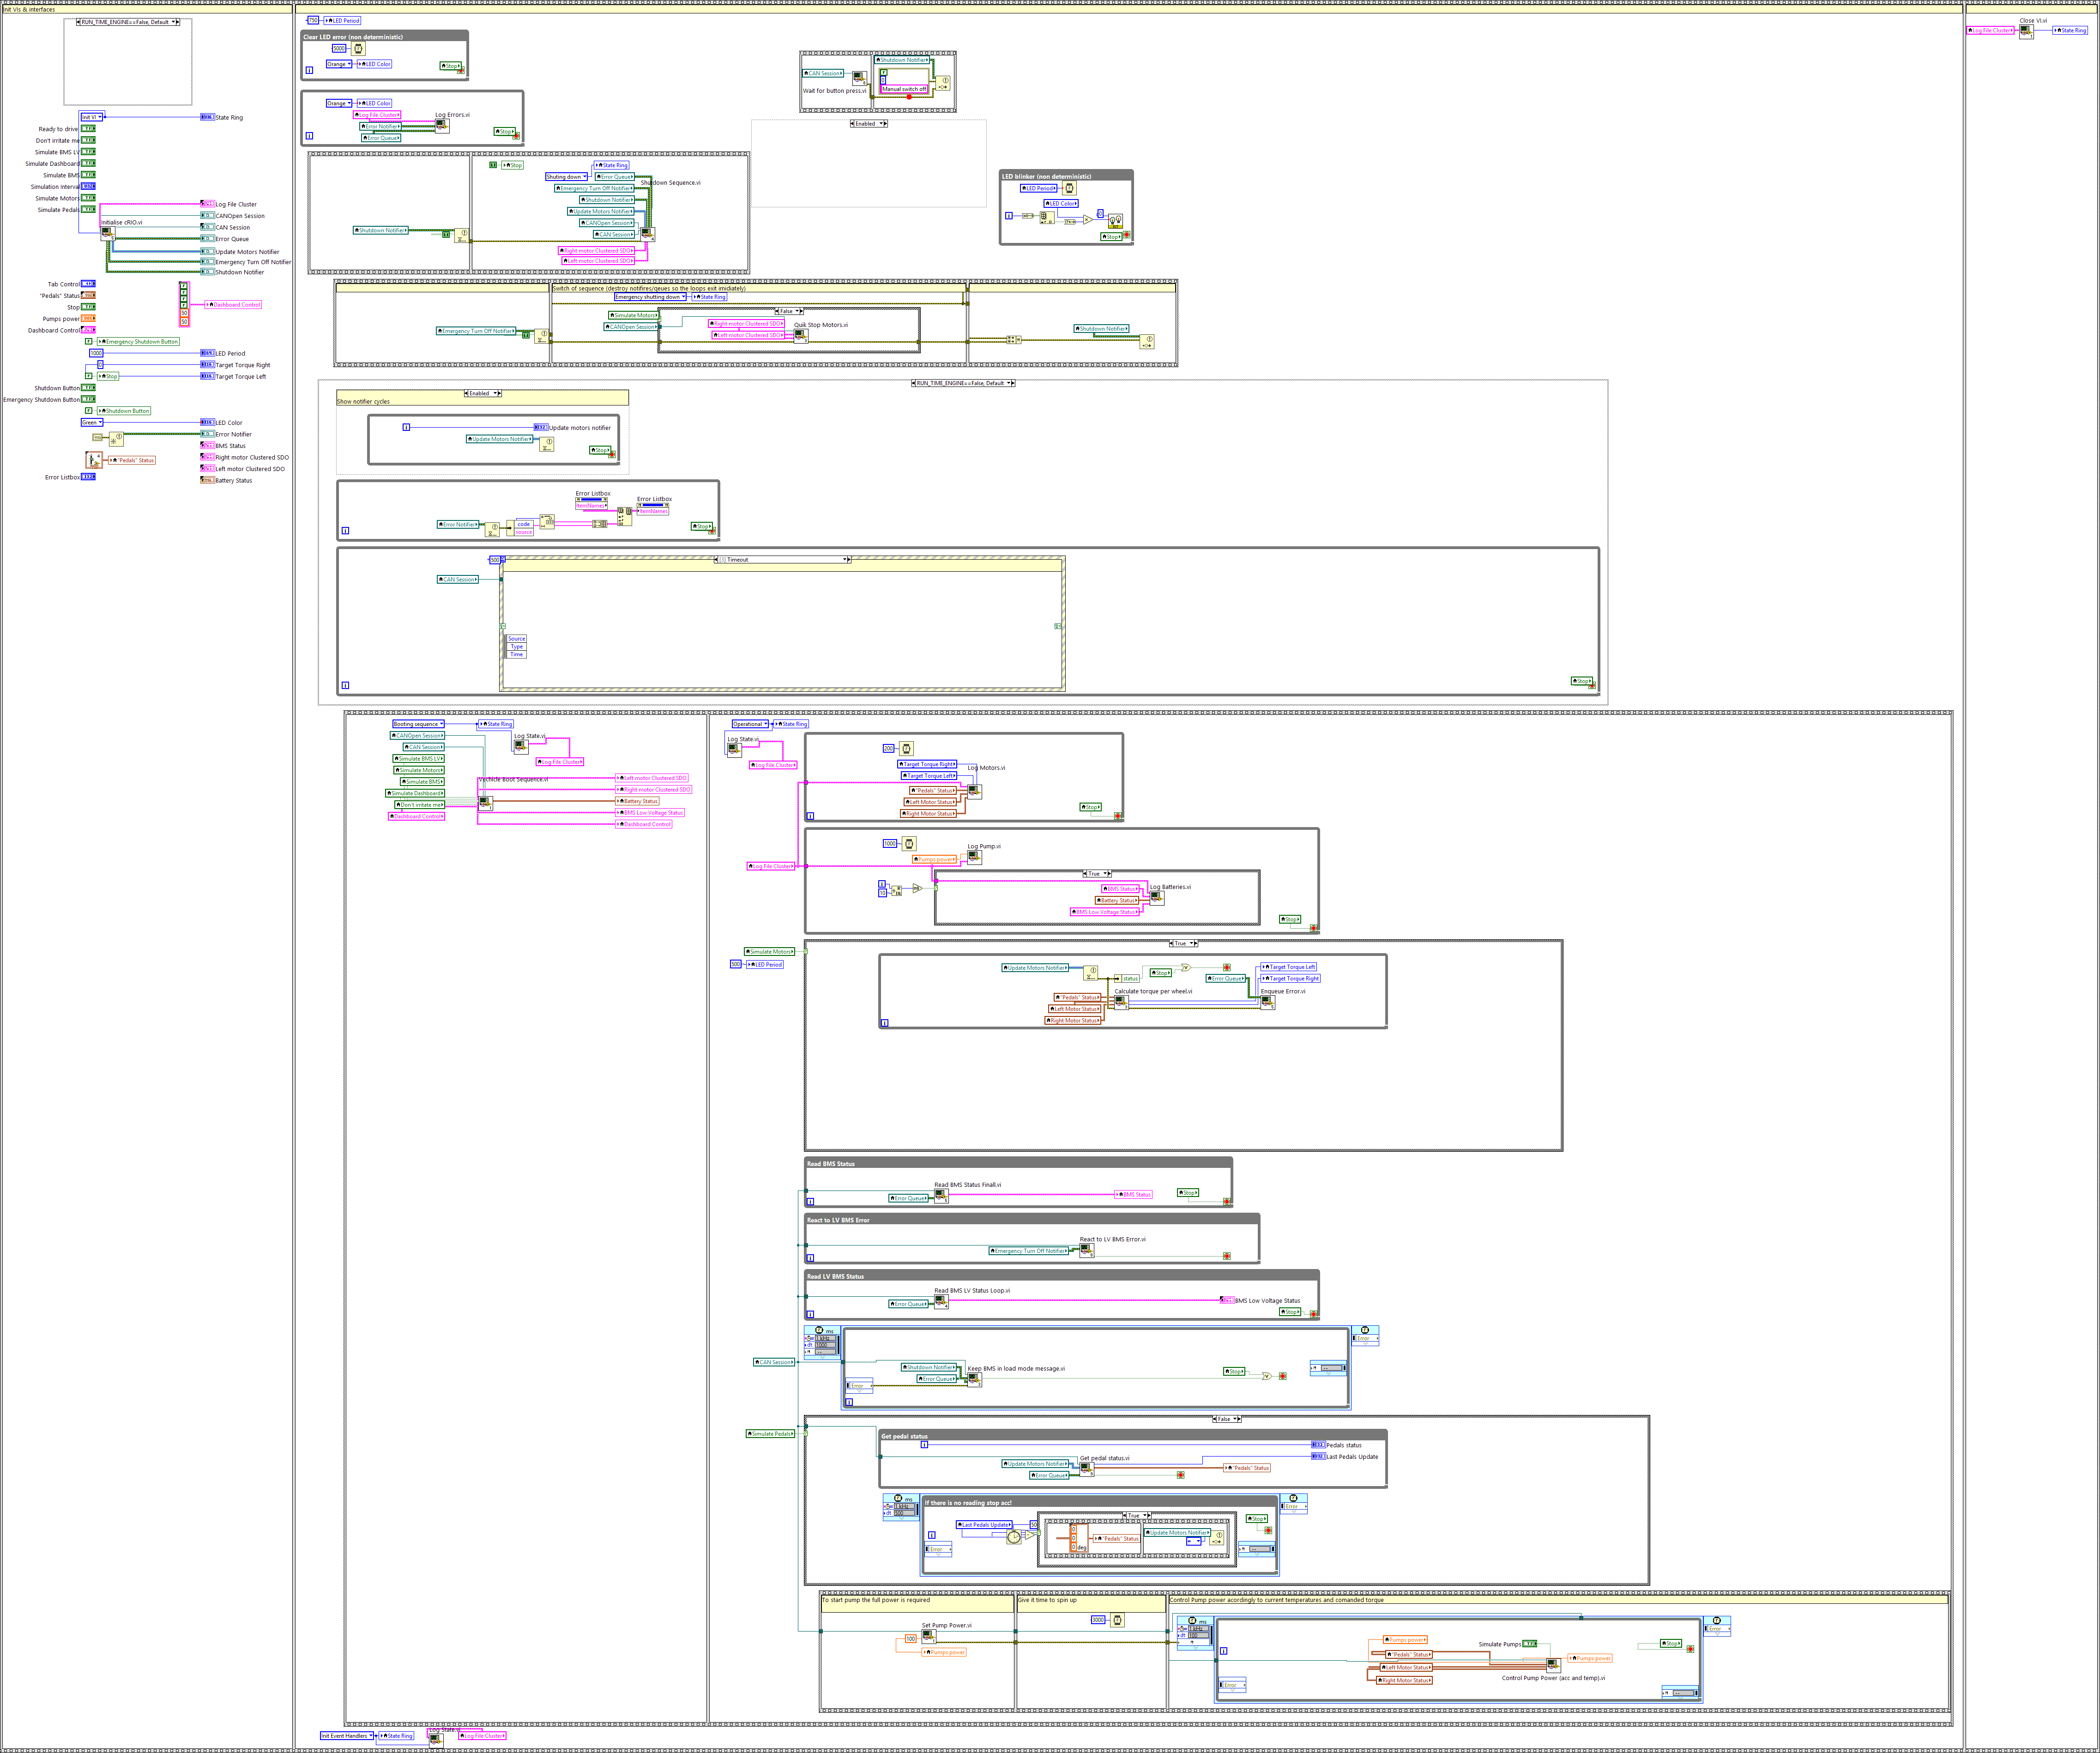
\includegraphics[width=\textwidth]{figures/Run_maind.png}
    \caption{main.vi}
    \label{vi:main}
\end{figure}

The main program is a sequence of stages which for simplicity I will call "Initialisation", "Operation" and "Closing". Out of 3, the last one has no complexity to be explained, its only function is to close the log file. 
I have tried to reflect each level of functionality nesting by the document structure Section->Subsection->Subsection->Paragraph etc. However, to avoid overwhelmingly deep nest structure I have elevated description of "Vehicle control - drive" from point \ref{sec:veh_contr} to separate section. Also I used the last section to describes low level functions which has been used in the whole project.

\section{Initialisation}
\begin{wrapfigure}{l}{0.33\textwidth}
    \centering
    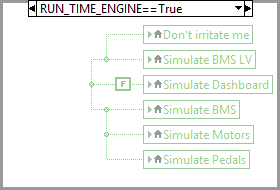
\includegraphics[width=0.3\textwidth]{figures/Run_maind31.png}
    \caption{Turn of simulation when used without control panel}
    \label{vi:maind31}
    \vspace{-15pt}
\end{wrapfigure}
Upon start internal initial values are set to avoid any non-deterministic behaviour. In case the program so called within open remote control panel the simulation switches are not reset so one can first setup desired modules to validate and turn one the simulation for the rest of them.
This has been done by sensing LabVIEW's "RUN\_TIME\_ENGINE" environmental value and setting simulation values to false (\ref{vi:maind31}).
\\ \\
\subsection{Initialise sub-modules}
\begin{wrapfigure}{!r}{0.33\textwidth}
    \vspace{-15pt}
    \centering
    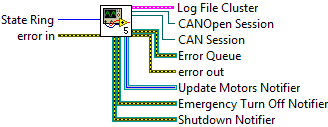
\includegraphics[width=0.3\textwidth]{figures/Initialise_cRIOc}
    \caption*{}
    \label{vi:init_crioc}
    \vspace{-15pt}
\end{wrapfigure}
Whenever setting of basic parameters is done the Initialise\_cRIO.vi is called to boot sub-modules, init the synchronisation primitives and start logging of system state (\ref{vi:init_crioc}).
\begin{figure}[!h]
    \centering
    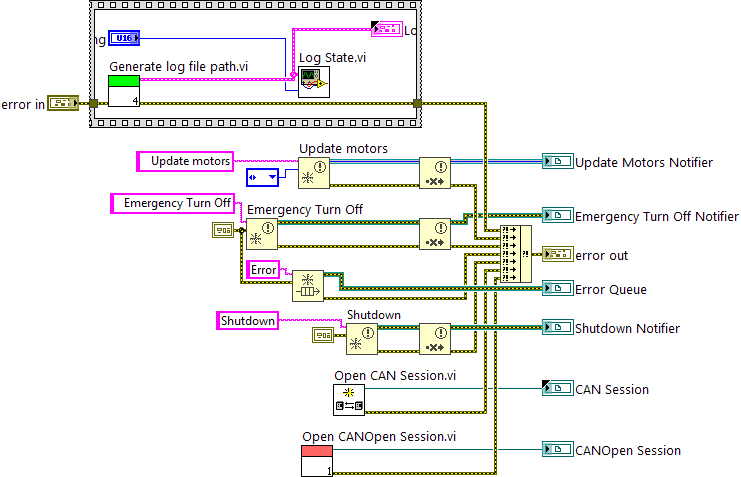
\includegraphics[width=\textwidth]{figures/Initialise_cRIOd.png}
    \caption{Initialise\_cRIO.vi}
    \label{vi:init_crioc}
\end{figure}

In the VI, three notifiers\footnote{LabVIEW synchronisation primitive acting in a similar way to interrupts} are spawned:
\begin{itemize}
    \item Update motors - motors should be updated with new data
    \item Emergency Turn Off - in case of motors should be stopped immediately
    \item Shutdown - turning off the controller
\end{itemize}
Additionally error queue is initialised which would accumulate the errors and similarly to notifies act like interrupt upon change\footnote{This synchronisation primitive act similarly to double linked list which raises interrupt upon any change}.

\subsubsection{Generate log file}
\begin{figure}[h]
    \centering
    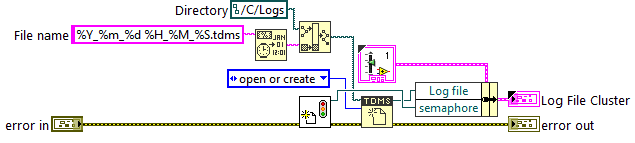
\includegraphics[width=\textwidth]{figures/Generate_log_file_pathd.png}
    \caption{Generate\_log\_file\_path.vi}
    \label{vi:Generate_log_file_path}
\end{figure}
Beside this, I the code calls Generate\_log\_file\_path.vi (\ref{vi:Generate_log_file_path}) which opens or creates log file within current date and time as a file name so it is easy to navigate and each time the car has been turned on is saved in separate log.
Additionally to acquiring the file handle the code also spawns semaphore to be used within it (the log file cannot be written simultaneously by multiple threads/processes).

Just after opening the log handle the current state of the device is saved.
\\ \\
Last but not least the Initialise\_cRIO.vi call the functions to start communication responsible sub-modules (CAN Session and CANOpen Session).
\subsubsection{Initialise CANOpen Session}
\begin{figure}[h]
    \centering
    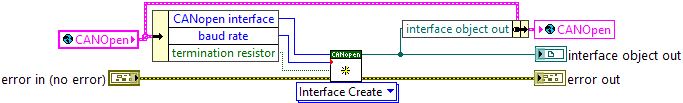
\includegraphics[width=\textwidth]{figures/Open_CANOpen_Sessiond}
    \caption{Open\_CANOpen\_Session.vi}
    \label{vi:Open_CANOpen_Session}
\end{figure}
National Instruments provides a great interface for their CANOpen module so starting the module is as easy as calling the associated function with proper parameters. 
\subsubsection{Initialise CAN}
On the other hand to interference with CAN module only very low-level API has been provided which on FPGA level is able to accept CAN frame to send and return read one. Therefore the whole interface needed to be built on the top of this API to provide all the data and usable abstraction from real-time processor level.
\begin{figure}[h]
    \centering
    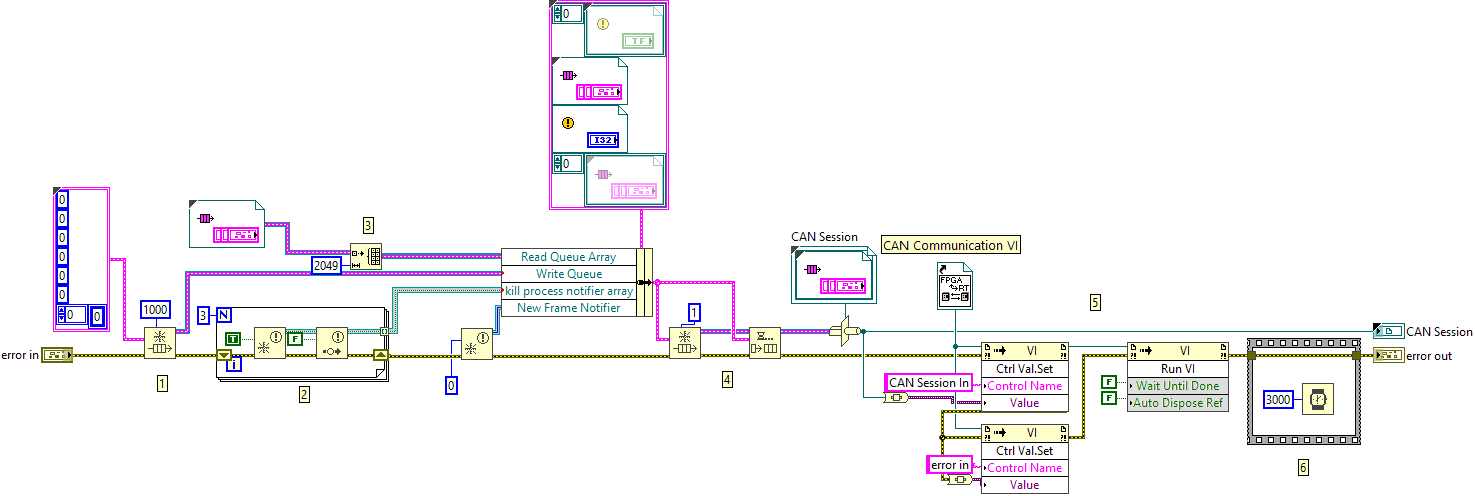
\includegraphics[width=\textwidth]{figures/Open_CAN_Sessiond}
    \caption{Open\_CAN\_Session.vi}
    \label{vi:Open_CAN_Session}
\end{figure}
Implementation would hard to discuss as whole so figure \ref{vi:Open_CAN_Session} has been enriched by indexing labels which following points refers to:
\begin{enumerate}
    \item As the first step, the queue (linked list) is created to serve as a buffer for messages to be written to the bus.
    \item Then notifiers/interrupts are defined so the interface can be gracefully closed.
    \item Array with entity for each message ID is created, as for the point of time it is filled with zero references to queues capable of containing CAN Frames\footnote{CAN Frame (instead of CAN frame) is used to signal that it refers to the data structure, not physical signal pattern} (queue with the data type set to be a CAN Frame).
    \\
    \todo{correct numbering}
    Initiate notifier/interrupt to be raised every time a new message would come.
    \item Encapsulate CAN session object so it can be passed around the code by reference.
    \item Execute the code servicing the CAN messages on FPGA (and passes it to RT processor).
    \item Wait to ensure that the FPGA was fully initiated by the time this function exits.
\end{enumerate}

\section{Operation}
Whenever all values and services are initialised device move into operational state and logs this change.
This stage defines all the tasks running in parallel during device operation. To start with the error logging loop is started so in case of any failure, it would be possible to reason of what has happened. 
For instant feedback whenever a remote panel is not connected the diode of cRIO is made to blink within an interval of 1,5s (50$\%$ duty cycle), changing its colour to orange for 5s seconds whenever the error has been encountered.\label{cRIO_LED}

\subsection{Shutdowns}
Then the shutdown functions are described as follows.
\begin{figure}[h]
    \centering
    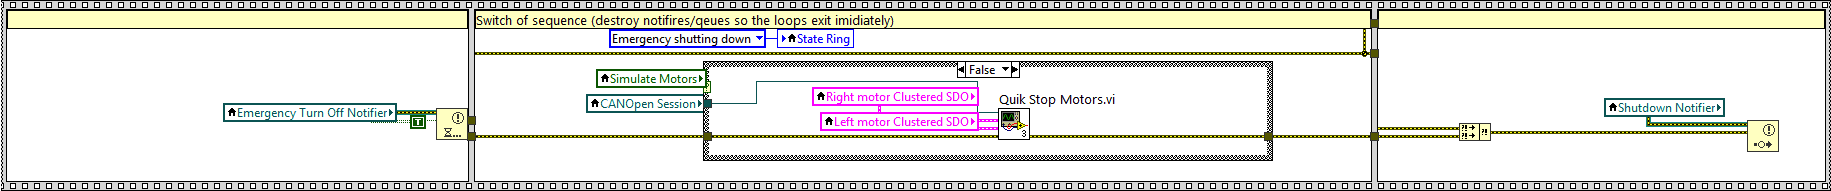
\includegraphics[width=\textwidth]{figures/Emergency_turn_off}
    \caption{Emergency shutdown}
    \label{vi:emc_shut}
\end{figure}
Emergency shutdown (\ref{vi:emc_shut}) react upon notification/interrupt and if the motors are not simulated the "Quick stop" message is sent to both of them. Then after possibly avoiding hazardous situation controller follows up with normal shutdown sequence (\ref{vi:shut}).
\begin{figure}[h]
    \centering
    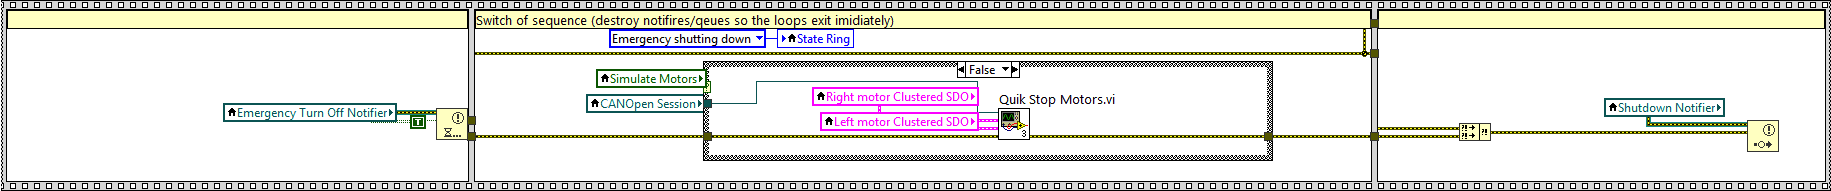
\includegraphics[width=\textwidth]{figures/Emergency_turn_off}
    \caption{Shutdown}
    \label{vi:shut}
\end{figure}

During normal shutdown process (\ref{vi:shut_seq})
\begin{figure}[h]
    \centering
    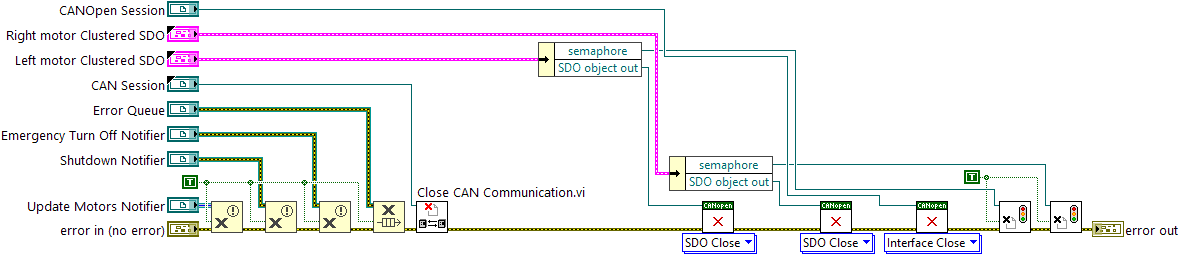
\includegraphics[width=\textwidth]{figures/Shutdown_Sequenced}
    \caption{Shutdown\_Sequence.vi}
    \label{vi:shut_seq}
\end{figure}
I start with deleting all the notifiers and error queue so if any thread/process function is waiting for them it would exit immediately.
Then the same needs to be done for next nested level - CAN session which I would describe in the next subsection.
Last but not least the CANOpen communication objects are released, CANOpen session closed and associated semaphores deleted. 

\subsubsection{Closing CAN}
Closing CAN session is a bit tedious task, analogue to opening process.
\begin{figure}[h]
    \centering
    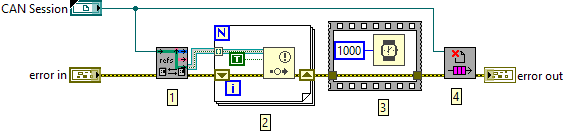
\includegraphics[width=\textwidth]{figures/Close_CAN_Communicationd}
    \caption{Close\_CAN\_Communication.vi}
    \label{vi:close_can}
\end{figure}
First of all the closing notifiers are acquired and close notifications send (point 2). This operation wound stop the receiving/sending loop. Once again to ensure that this already happened we are waiting a second. Then function is called to close all the primitives opened during initialisation process (\ref{vi:close_can_queues}).
\begin{figure}[h]
    \centering
    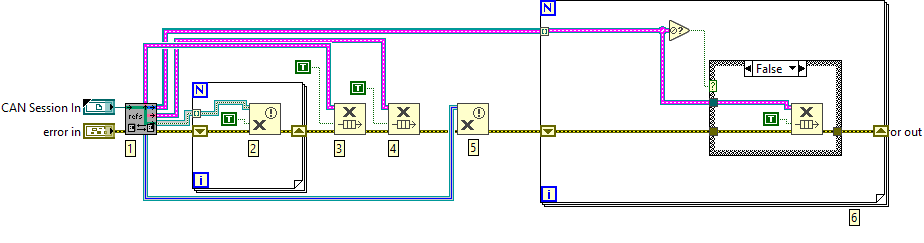
\includegraphics[width=\textwidth]{figures/Close_CAN_Communication_queuesd}
    \caption{Close\_CAN\_Communication\_queues.vi}
    \label{vi:close_can_queues}
\end{figure}
\begin{enumerate}
    \itemsep0.1em 
    \item CAN Session is cast back to object.
    \item Shutdown notifiers are being deleted.
    \item The queue used to encapsulate the session is deleted.
    \item The queue containing messages to be sent is deleted.
    \item Deleting new frame notifier
    \item Last but not least iterate over all message IDs and delete associated queues.
\end{enumerate}

\subsection{Debugging loops}
For the time of development and whenever the program is run within a remotely controlled session. I implemented functionality which helps in debugging of any system misbehaviour.

One of the important indicators is the live number of interrupts to update motor values. Also, errors, if any, are shown in pleasant to use list. However, different functionality plays a key role in here.

In the remote session, I have provided visual indicators for subsystems. Moreover, I have provided bindings so the devices can be using a real data or be simulated.

\begin{figure}[h]
    \centering
        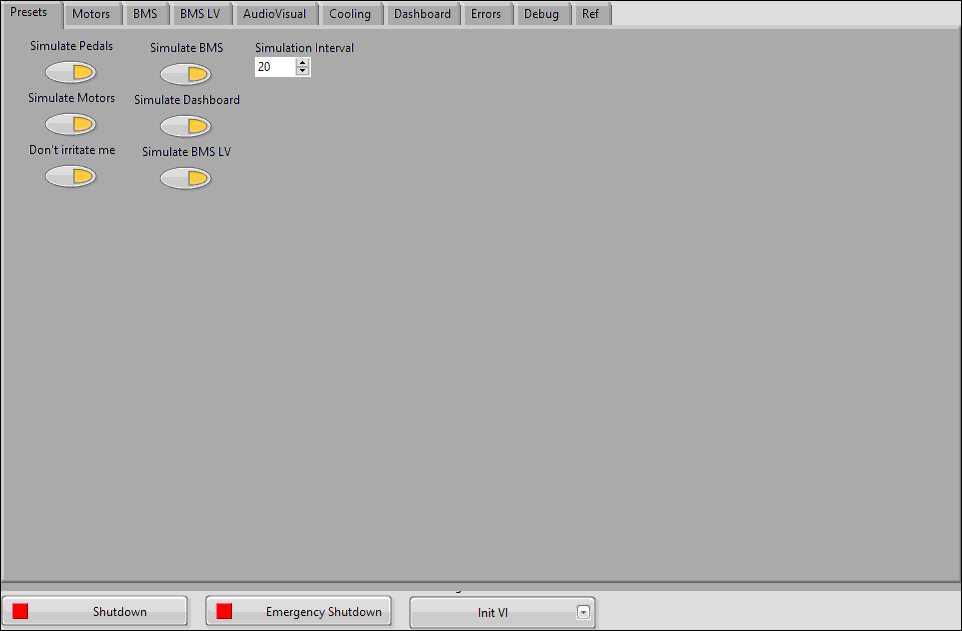
\includegraphics[height=5cm]{figures/Run_mainp0.png}
        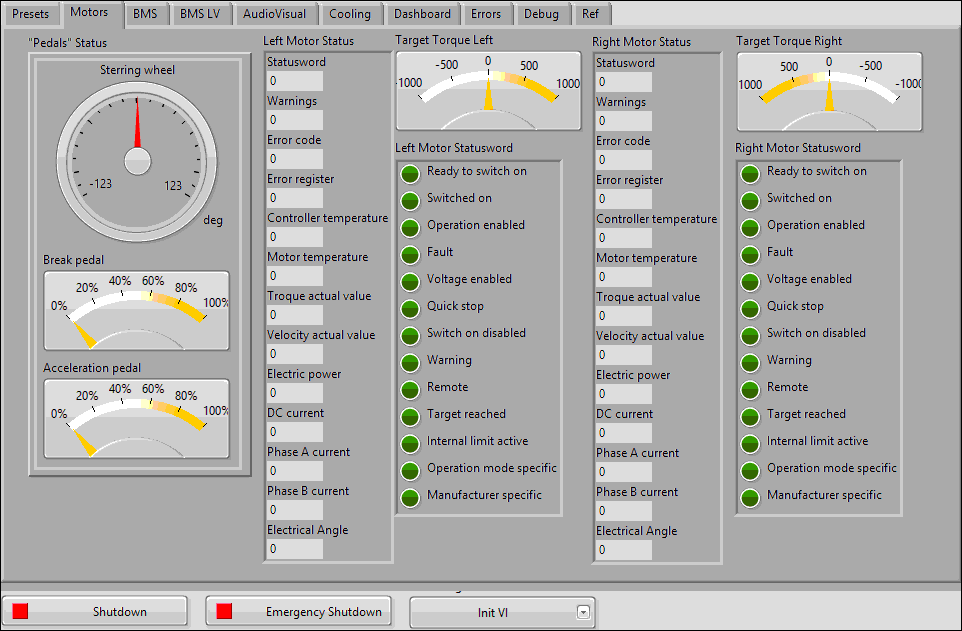
\includegraphics[height=5cm]{figures/Run_mainp1.png}
\end{figure}
\begin{figure}[h]\ContinuedFloat
    \centering
        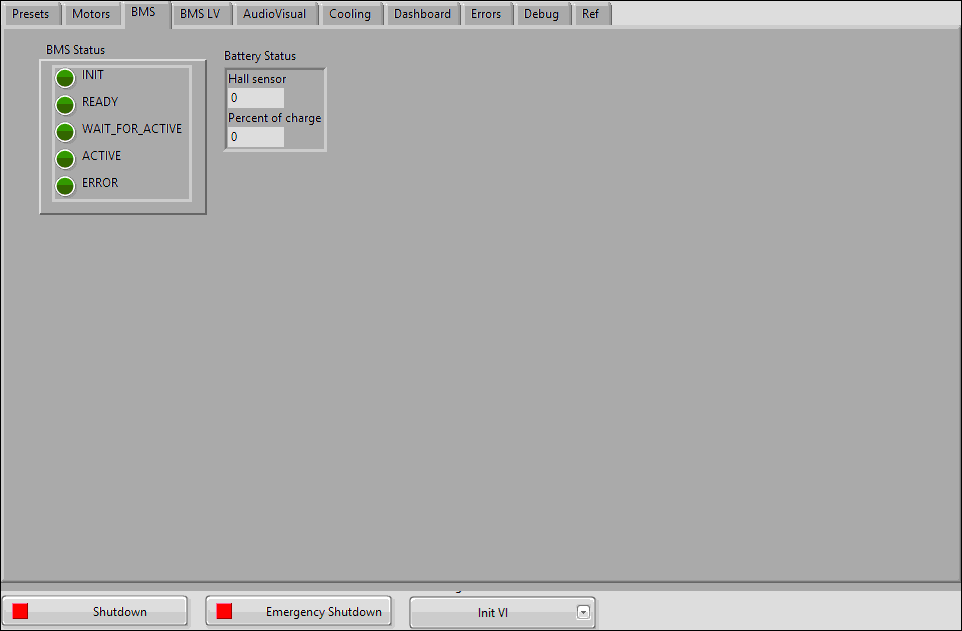
\includegraphics[height=5cm]{figures/Run_mainp2.png}
        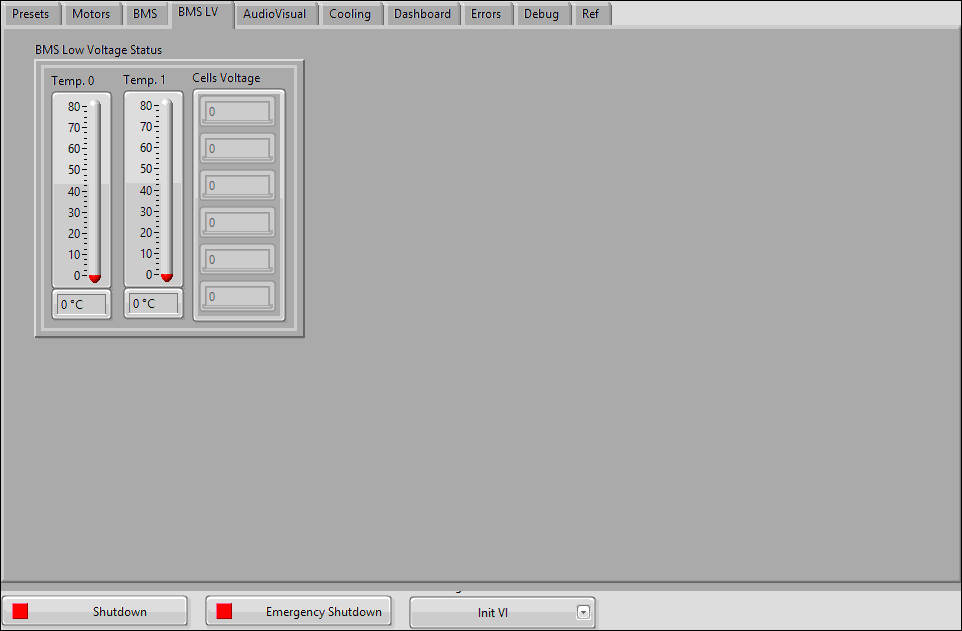
\includegraphics[height=5cm]{figures/Run_mainp3.png}
\end{figure}
\begin{figure}[h]\ContinuedFloat
    \centering
        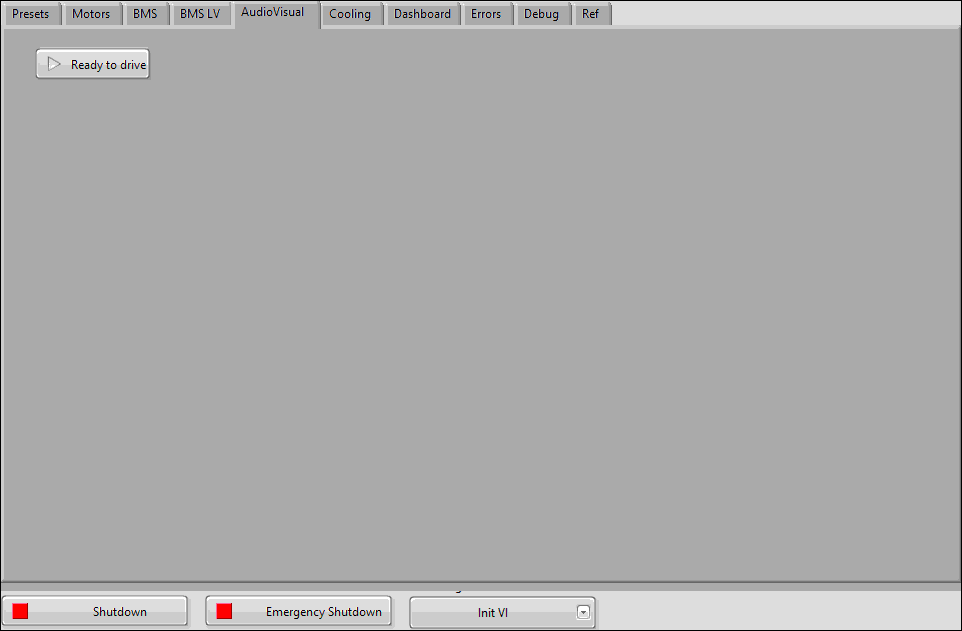
\includegraphics[height=5cm]{figures/Run_mainp4.png}
        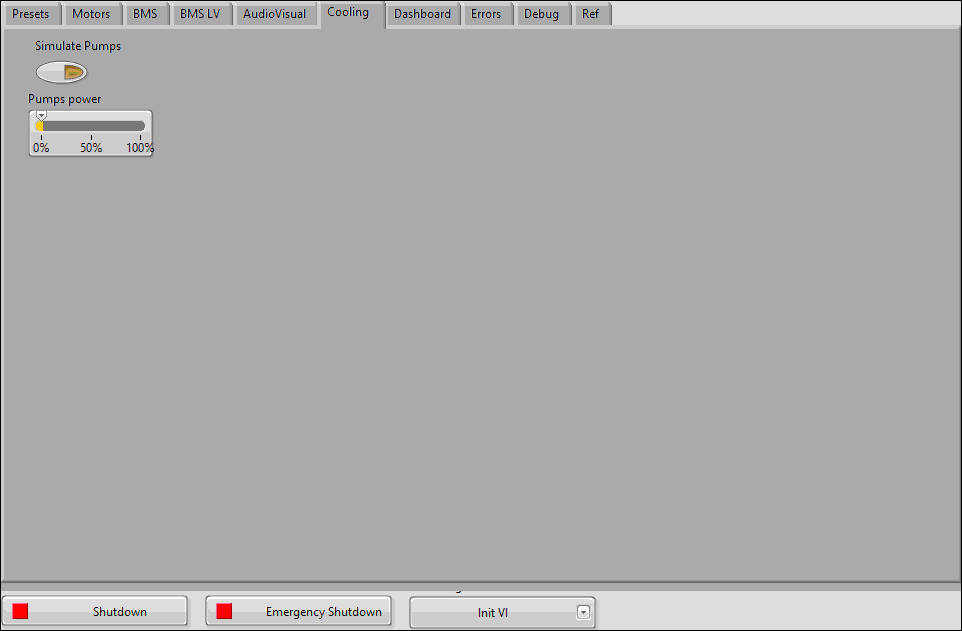
\includegraphics[height=5cm]{figures/Run_mainp5.png}
\end{figure}
\begin{figure}[h]\ContinuedFloat
    \centering
        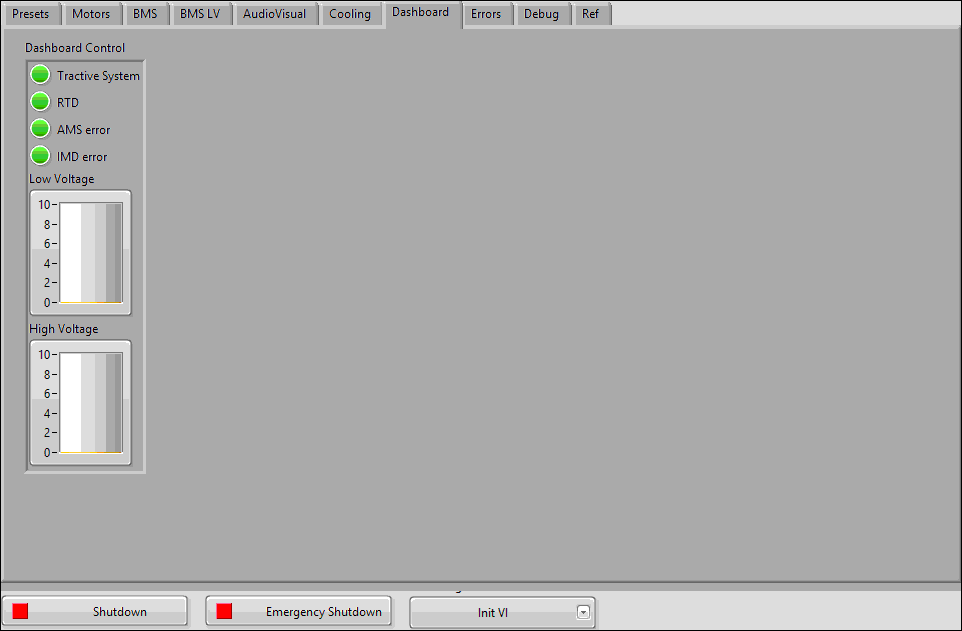
\includegraphics[height=5cm]{figures/Run_mainp6.png}
        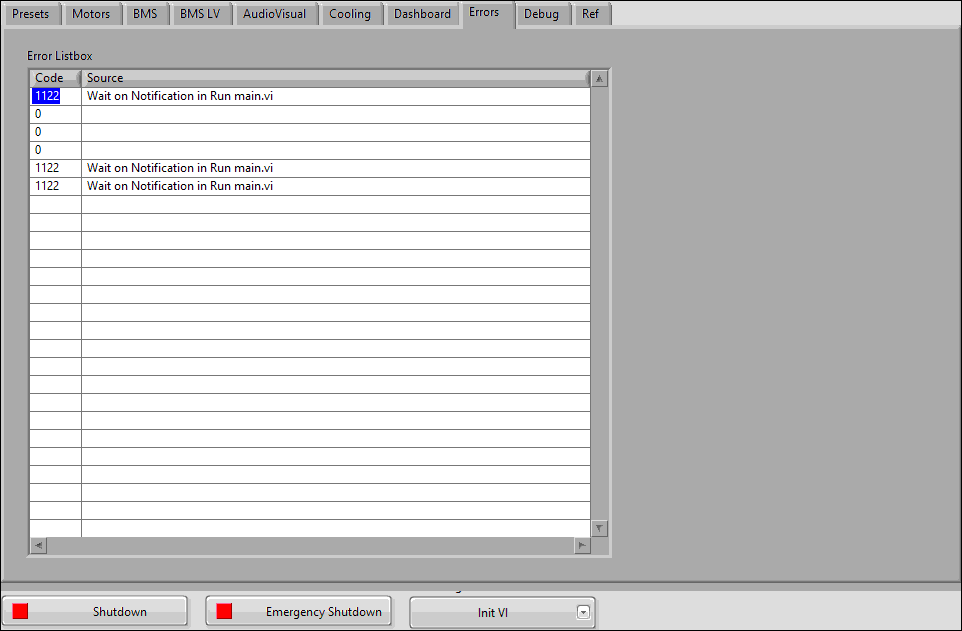
\includegraphics[height=5cm]{figures/Run_mainp7.png}
        \caption{Remote control user interface}
\end{figure}

Taking for example steering/pedals sensor, it is important to drive to motors in a controlled manner so while any changes to sensors have been done they might be tested with motors in simulation mode (the values are updated but motors are not spinning).

On the other hand, one might want to control the motors by remote session. To make so it is sufficient to just flip the switch responsible for pedals sensor simulation. Now the pedals indicator is acting as a control so a user might just grab the indicator needle and change the value in the system.

\subsection{Vehicle control}\label{sec:veh_contr}
The vehicle control consists of two steps. First follows the sequence required to safely boot the motor controllers (apply high voltage/current). Second to control vehicle while operational - drive.

\subsubsection{Boot sequence}
Starting code has been shown in figure \ref{vi:boot_sequence}
\begin{figure}[H]
    \centering
    \renewcommand{\thesubfigure}{}% no subfigure number
    \tightsubcaptions % we want tight subcaptions
    \setlength{\subfloatlabelskip}{0pt}% no space between number and caption
    \subbottom[Part 1]{
        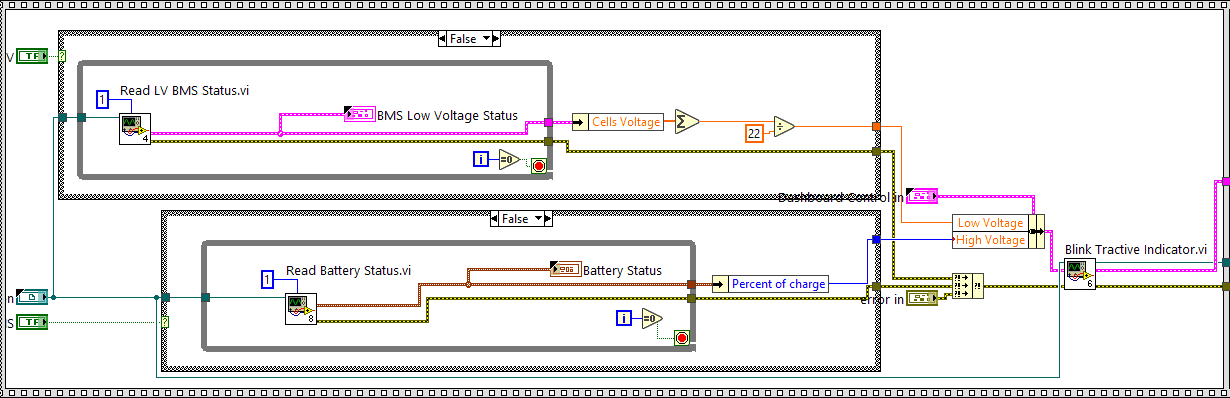
\includegraphics[width=\textwidth]{figures/Vechicle_Boot_Sequenced01}
    }
\end{figure}
\begin{figure}[H]\ContinuedFloat
    \centering
    \renewcommand{\thesubfigure}{}% no subfigure number
    \tightsubcaptions % we want tight subcaptions
    \setlength{\subfloatlabelskip}{0pt}% no space between number and caption
    \subbottom[Part 2]{
        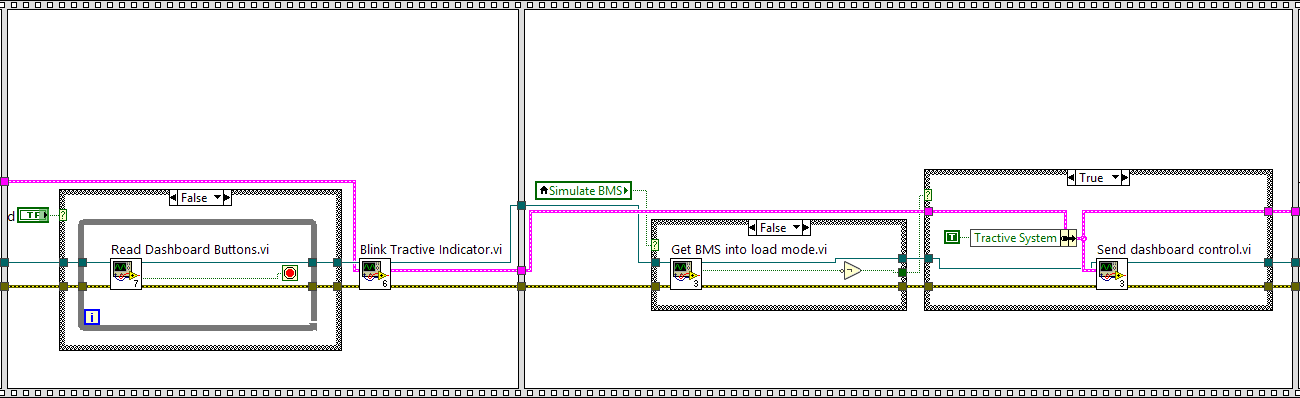
\includegraphics[width=\textwidth]{figures/Vechicle_Boot_Sequenced02}
    }
\end{figure}
\begin{figure}[H]\ContinuedFloat
    \centering
    \renewcommand{\thesubfigure}{}% no subfigure number
    \tightsubcaptions % we want tight subcaptions
    \setlength{\subfloatlabelskip}{0pt}% no space between number and caption
    \subbottom[Part 3]{
        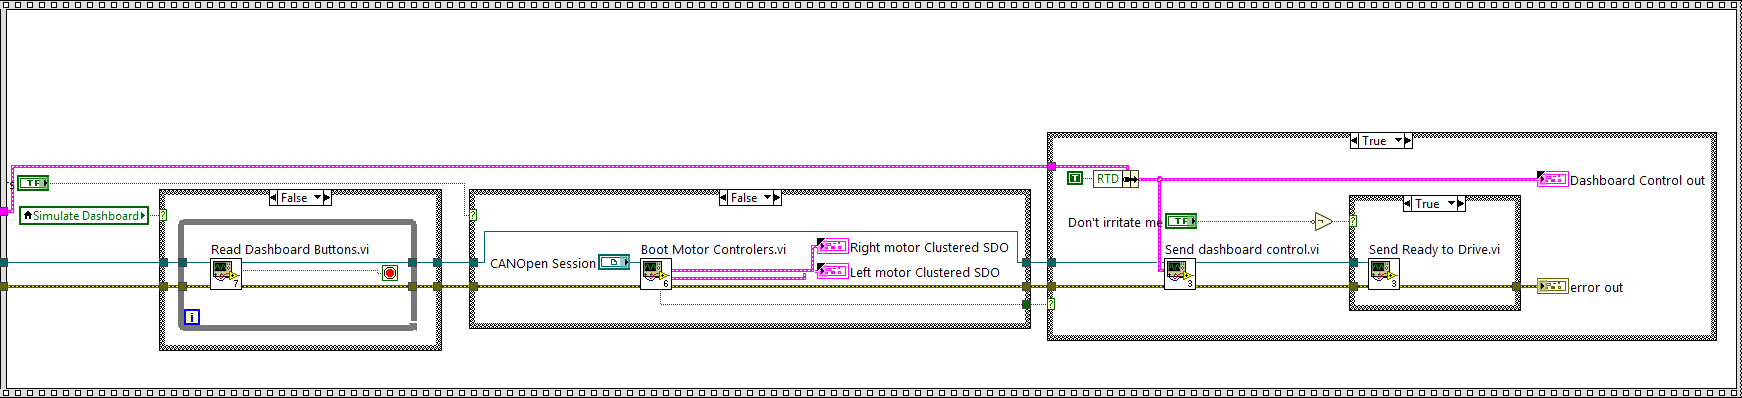
\includegraphics[width=\textwidth]{figures/Vechicle_Boot_Sequenced03}
    }
    \caption{Vehicle\_boot\_sequence.vi}
    \label{vi:boot_sequence}
\end{figure}
it can easily be describe in a few consecutive points:
\begin{enumerate}
    \itemsep0.1em 
    \item Firstly it tries\footnote{within 1s timeout, after which default values are assumed. Error would be not crucial for functioning of vehicle so it is ignored} to read state of charge form low voltage and main BMS based on which dashboard indicators are updated.
    \item Wait for ignition button (marked TS - Tractive System) to be pressed and blink it as acknowledge upon push.
    \item Get BMS into load mode (further described in next section) and turn traction active indicator on upon success.
    \item Wait for ready to drive (RTD) button to be pressed.
    \item Turn motor controllers into drive mode (further described in section \todo{ref}).
    \item In case of success turn on the RTD indicator and send command to audio-visual subsystem to make ready to drive notification sound.
\end{enumerate}

\paragraph{Turning on BMS}
\begin{figure}[H]
    \centering
    \renewcommand{\thesubfigure}{}% no subfigure number
    \tightsubcaptions % we want tight subcaptions
    \setlength{\subfloatlabelskip}{0pt}% no space between number and caption
    \subbottom[Part 1]{
        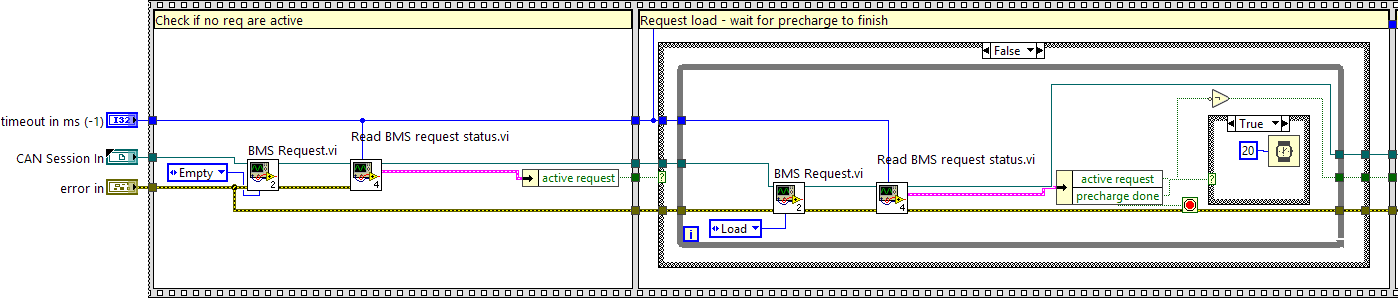
\includegraphics[width=\textwidth]{figures/Get_BMS_into_load_moded01}
    }
\end{figure}
\begin{figure}[H]\ContinuedFloat
    \centering
    \renewcommand{\thesubfigure}{}% no subfigure number
    \tightsubcaptions % we want tight subcaptions
    \setlength{\subfloatlabelskip}{0pt}% no space between number and caption
    \subbottom[Part 2]{
        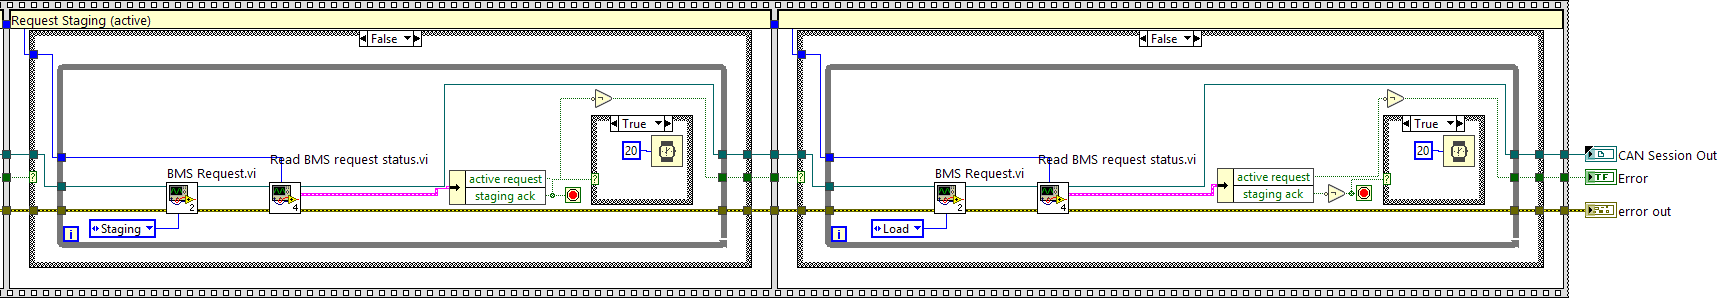
\includegraphics[width=\textwidth]{figures/Get_BMS_into_load_moded02}
    }
    \caption{Get\_BMS\_into\_load\_mode.vi}
    \label{vi:boot_BMS}
\end{figure}
While contacting with BMS I firstly ensure that BMS is in initial mode by checking its status. Then BMS is requested to turn on into load mode withing ~20ms interval until the pre-charge process is done. Then BMS is moved to staging process and active load letter one.

Reasoning behind this sequence has been described in BMS manual \cite{BMS_manual}.

\paragraph{Boot motor controller}
\begin{figure}[H]
    \centering
    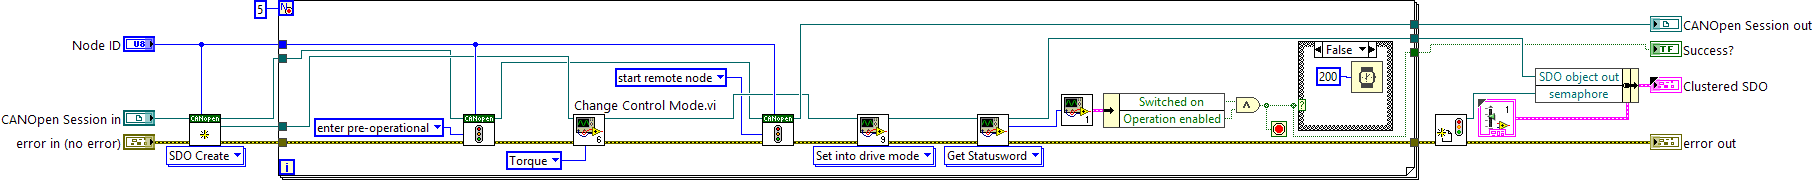
\includegraphics[width=\textwidth]{figures/Boot_Motor_Controlerd}
    \caption{Boot\_motor\_controller.vi}
    \label{vi:boot_MC}
\end{figure}
The code performs up to five tries to get motor controller into a operational mode (within 200ms delay in between). On each try the same sequence is repeated corresponding to path marked red in figure \ref{fig:em500_states}.
\begin{enumerate} 
    \itemsep0.1em 
    \item CANOpen command is send to move into pre-operational state.
    \item Set emDrive500 control mode to torque.
    \item Set "Mode of operation" to torque.
    \item CANOpen state change into operational.
    \item emDrive control word is set to "Fault reset" -> Shutdown -> Switch on + operation enable.
    \item Get status word to to ensure proper state (in case of fail, repeat).
\end{enumerate}

Whenever the controllers are finally operational the SDO communication object handle is saved within semaphore which will be used to ensure that it is not used by many threads in parallel (NI CANOpen library limitation).

\vspace{1em}
\noindent\fbox{%
    \parbox{\textwidth}{%
        For simplicity and to emphasise importance the sub-subsection "Vehicle control - drive" has been moved from its logical placement in here to separate section.
    }%
}

\section{Vehicle control - drive}
To start with event of entering the next state is saved into log file and the LED indicator pattern is changed (v.s.\ref{cRIO_LED}). The vehicle control for its drive mode spawns additional loops in parallel the the ones already started during initialisation.

\subsection{Logging}
Two of them are simply responsible for logging the device state (figure \ref{logging}).
\begin{figure}[H]
    \centering
    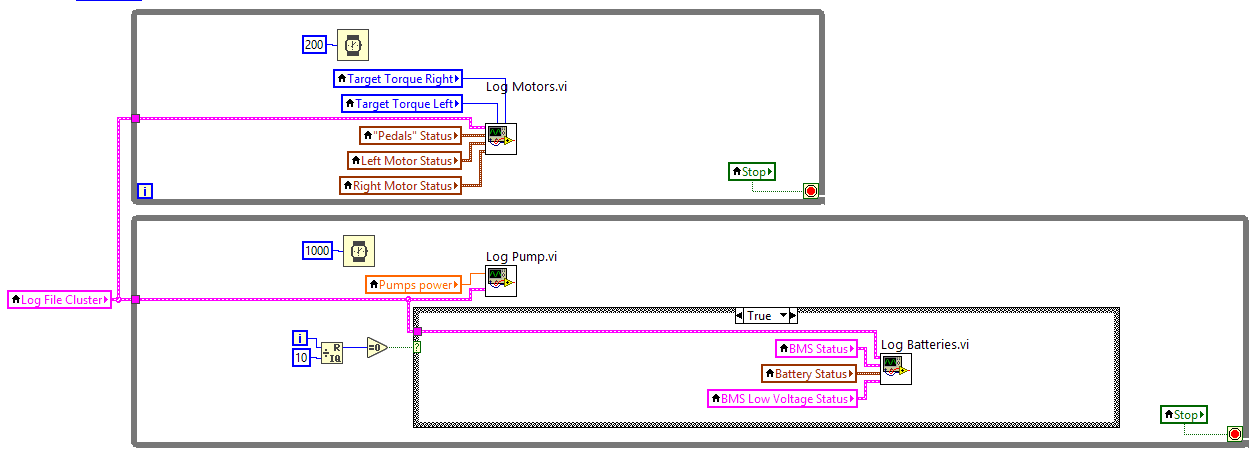
\includegraphics[width=\textwidth]{figures/Drive_log.png}
    \caption{Logging}
    \label{logging}
\end{figure}
Logging has been made in loops with non-deterministic timing where the current motor, pedal status and the associated control values are saved withing interval of 200ms.
Whereas slow changing signals as pump status is saved on each second and the batteries state is logged with period of 10s.

\subsection{Service BMS}
Then there are loops to read (and update local value) of low voltage BMS status and react to its error. As well as one to read main BMS status.
\begin{figure}[H]
    \centering
    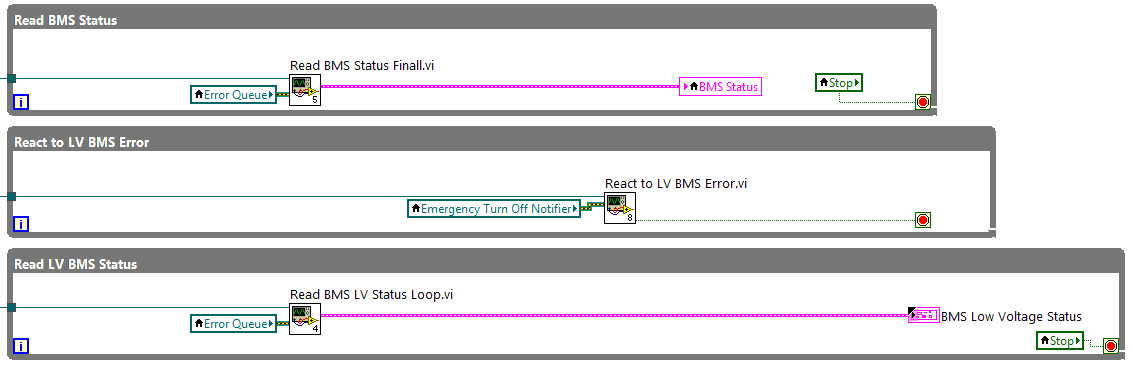
\includegraphics[width=\textwidth]{figures/Read_BMSs.png}
    \caption{Service BMS messages}
    \label{BMSs_status}
\end{figure}
To keep the BMS in load mode it needs to receive load request at least once per two seconds\footnote{Adjustable value, default used in the setup} so, since it is not a cost-full operation, to have an error margin the code was setup to send this message once per second.
Additionally this loop has been used to actually sense if the BMS is in load mode and turn off the system otherwise (fig. \ref{vi:Keep_BMS_in_load_mode_message}).
\begin{figure}[H]
    \centering
    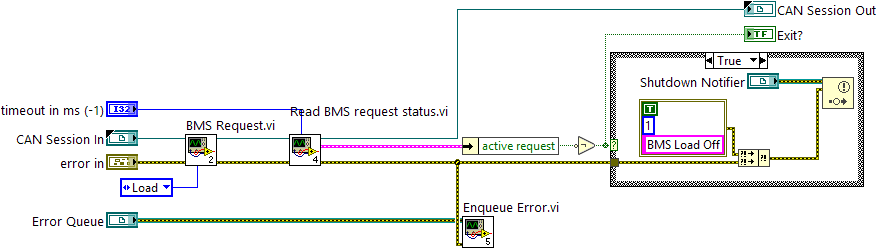
\includegraphics[width=\textwidth]{figures/Keep_BMS_in_load_mode_messaged}
    \caption{Keep\_BMS\_in\_load\_mode\_message.vi}
    \label{vi:Keep_BMS_in_load_mode_message}
\end{figure}

\subsection{Service steering wheel and pedals updates}
Pedals service beside simply receiving status messages and issuing messages to motors had to be enforced for the case when the communication is lost. Especially dangerous example is if accelerator pedal would be pressed down while communication got lost.
In the most simple approach car would keep accelerating until reaching to speed or it has been turned off.
\begin{figure}[H]
    \centering
    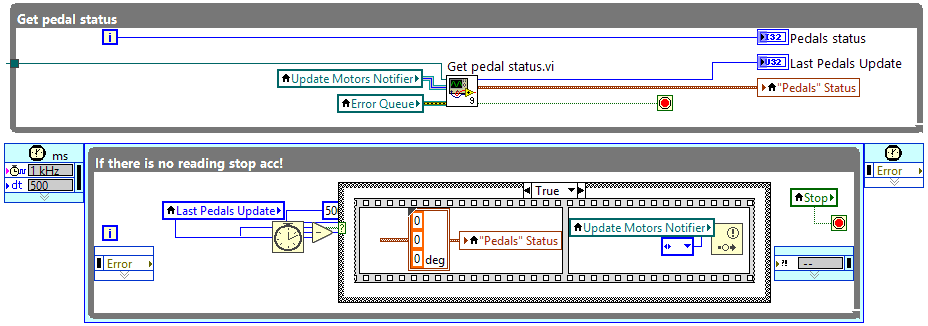
\includegraphics[width=\textwidth]{figures/Pedals_status}
    \caption{Steering/pedals sensors service}
    \label{pedals_service}
\end{figure}
To counteract this unlikely event a watchdog like functionality has been implemented (fig. \ref{pedals_service}). Whenever within last 500 ms no sensors status has been read their values are reset to zeros and request for motors update is requested.

\subsection{Service motor controllers}
\begin{figure}[H]
    \centering
    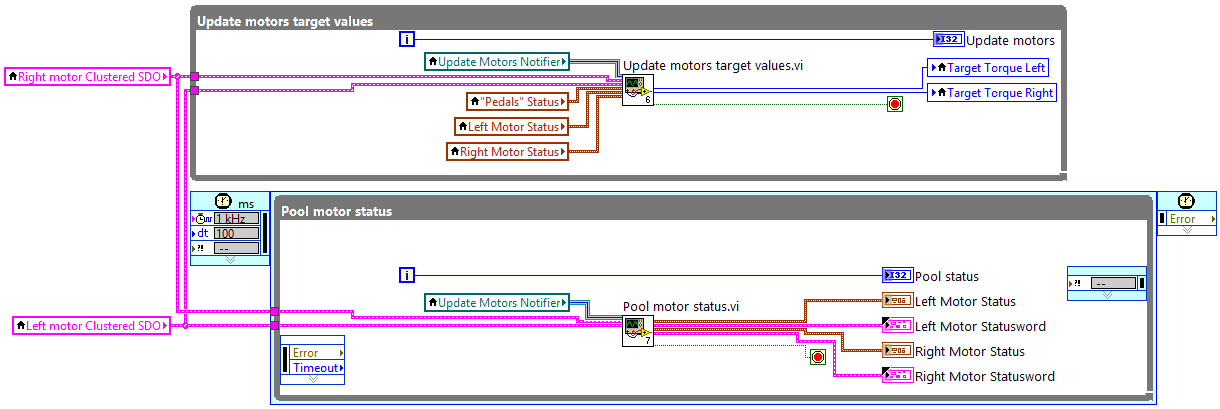
\includegraphics[width=\textwidth]{figures/Run_maind1_e}
    \caption{Service motor controllers}
    \label{s_m_c}
\end{figure}
\paragraph{Motor controller} target torque is updated on each request (notification in "Update Motors Notifier"). 
\begin{figure}[H]
    \centering
    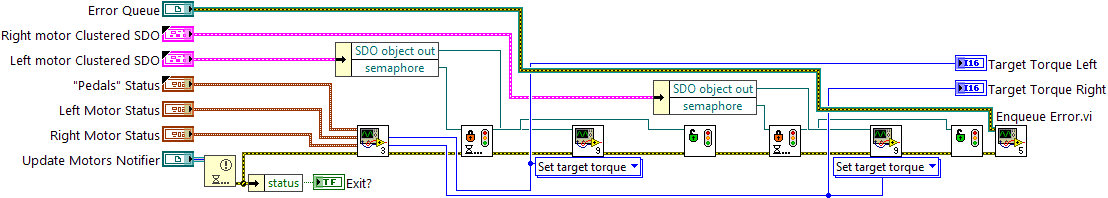
\includegraphics[width=\textwidth]{figures/Update_motors_target_valuesd}
    \caption{Update\_motors\_target\_values.vi}
    \label{vi:Update_motors_target_values}
\end{figure}
It is done in the manner that whenever \textit{Update\_motors\_target\_values.vi} is called it waits for notification. Then based current motors status and sensors value the target torque for each wheel is calculated (\todo{ref low level}). The communication object semaphore for one motor controller is obtained, value updated and semaphore released and the same is repeated for the other controller.

\\

\paragraph{Motor status} is obtained on each 100 ms by the call to Pool\_motor\_status.vs (fig. \ref{vi:Pool_motor_statusd}) which works in very similar manner to the way the target values are updated.
\begin{figure}[H]
    \centering
    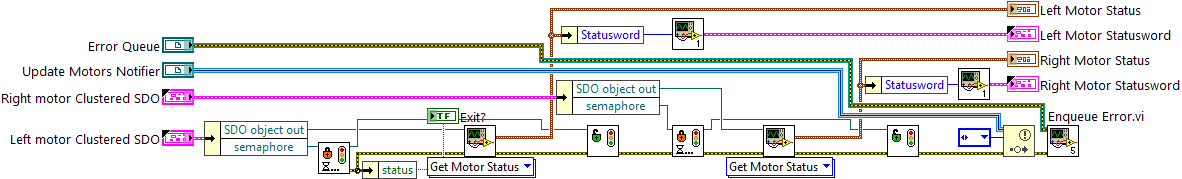
\includegraphics[width=\textwidth]{figures/Pool_motor_statusd}
    \caption{Pool\_motor\_status.vi}
    \label{vi:Pool_motor_statusd}
\end{figure}

\subsection{Service Pumps}
Last but not least during the drive mode the pumps are controlled by the code shown in figure \ref{pumps_service}.
\begin{figure}[H]
    \centering
    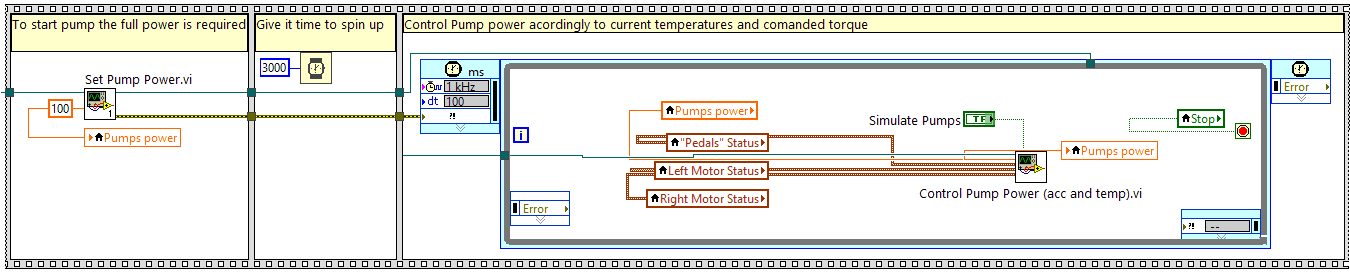
\includegraphics[width=\textwidth]{figures/Pumps}
    \caption{Pumps service}
    \label{pumps_service}
\end{figure}
What is happening in the code is that pumps are set to full power for first 3s (initialise spin) and the loop is started which updates pumps duty cycle based speed and motor temperatures on each 100ms.
The update is done by call to \textit{Control\_Pump\_Power\_(acc\_and\_temp).vi} which simply calculates desired duty cycle and sends the message to pump controller (VIs further described in \todo{ref}).
\begin{figure}[H]
    \centering
    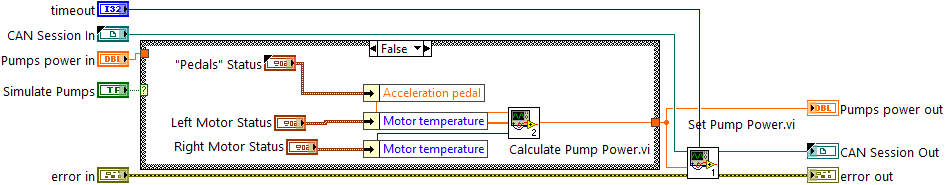
\includegraphics[width=\textwidth]{figures/Control_Pump_Power_(acc_and_temp)d_e}
    \caption{Control\_Pump\_Power\_(acc\_and\_temp).vi}
    \label{vi:Control_Pump_Power_(acc_and_temp)}
\end{figure}

\section{Low level API}
\subsection{Logging}
In quiet few places I have been using a special functions to log data, especially logging application state has been used through the whole application.
I have written 5 logging functions where all of them follows the same pattern.
\begin{figure}[h]
    \centering
    \renewcommand{\thesubfigure}{}% no subfigure number
    \tightsubcaptions % we want tight subcaptions
    \setlength{\subfloatlabelskip}{0pt}% no space between number and caption
    \subbottom[(a) Log\_State.vi]{
        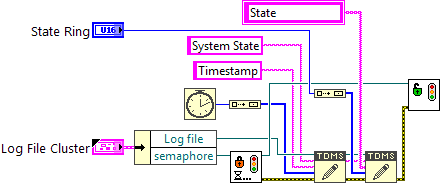
\includegraphics[width=0.36\textwidth]{figures/Log_Stated}
    }
    \subbottom[(b) Log\_Error.vi]{
        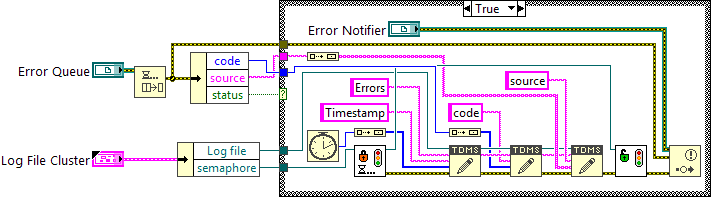
\includegraphics[width=0.56\textwidth]{figures/Log_Errorsd}
    }
\end{figure}
\begin{figure}[h]\ContinuedFloat
    \centering
    \renewcommand{\thesubfigure}{}% no subfigure number
    \tightsubcaptions % we want tight subcaptions
    \setlength{\subfloatlabelskip}{0pt}% no space between number and caption
    \subbottom[(c) Log\_Motor.vi]{
        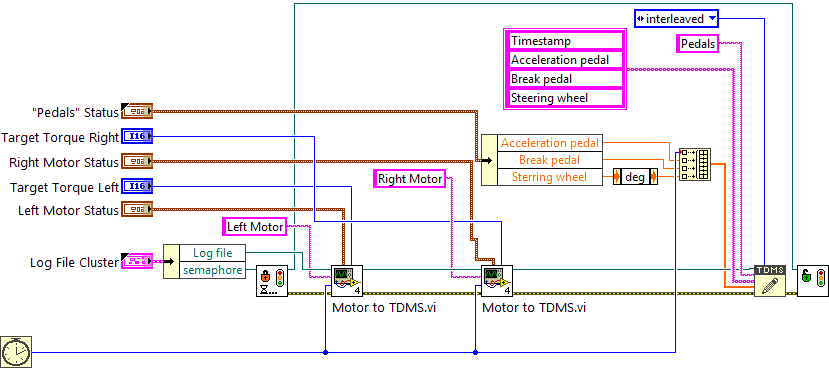
\includegraphics[width=0.56\textwidth]{figures/Log_Motorsd}
    }
    \subbottom[(d) Log\_Pump.vi]{
        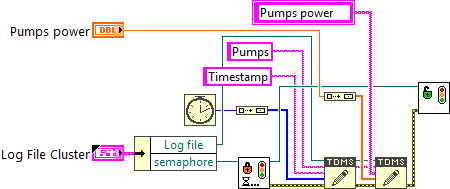
\includegraphics[width=0.36\textwidth]{figures/Log_Pumpd}
    }
\end{figure}
\begin{figure}[h]\ContinuedFloat
    \centering
    \renewcommand{\thesubfigure}{}% no subfigure number
    \tightsubcaptions % we want tight subcaptions
    \setlength{\subfloatlabelskip}{0pt}% no space between number and caption
    \subbottom[(e) Log\_Batteries.vi]{
        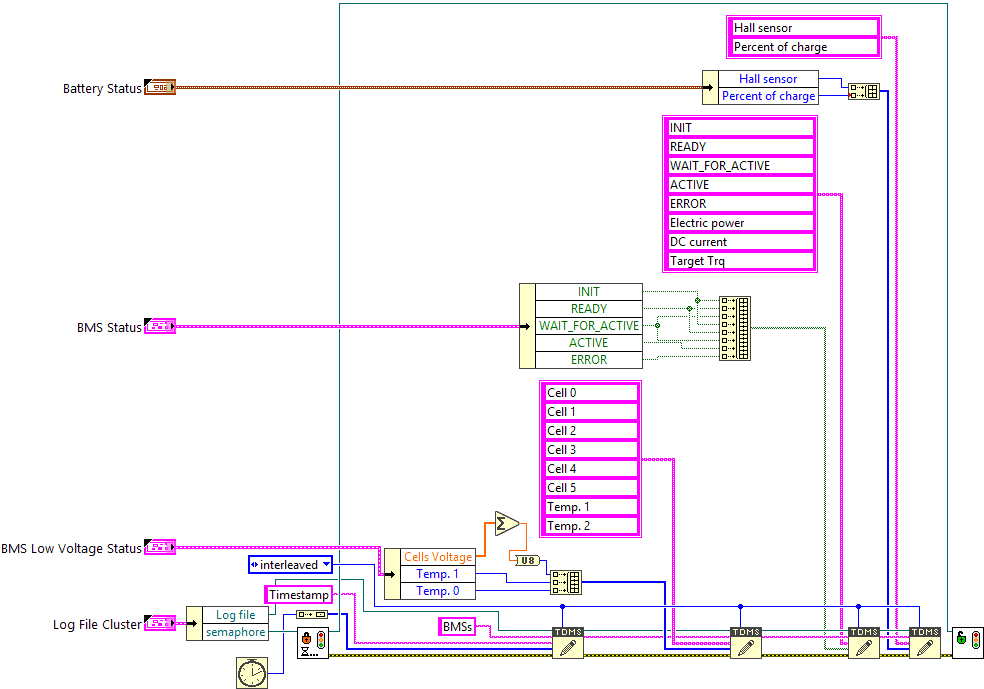
\includegraphics[width=\textwidth]{figures/Log_Batteriesd}
    }
    \caption{Logging functions}
\end{figure}
The semaphore for log file is acquired, then the data is save to TDMS file along with current time-stamp and semaphore is released. What is probably worth to mention is the split into few calls for TDMS write. The reason for it is that on single write only the array containing one type of data can be written, if one would try for instance write 8bit value along with 64bit one both would be saved as 64 numbers. To avoid this but also possibly limit the calls values has been grouped into arrays of the same type. For instance in \textit{Log\_Betteries.vi} first time-stamp is saved (it has corresponding type in TDMS format), then the array of 8bit values from low voltage BMS, soon after follows Boolean array from BMS status and last but not least two 32-bit values from battery status.

The same procedure has been followed has been followed in all the files including \textit{Log\_Motors.vi} where it has been implemented in separate file to avoid duplication - \textit{Motor\_to\_TDMS.vi} (fig. \ref{vi:Motor_to_TDMS}).
\begin{figure}[H]
    \centering
    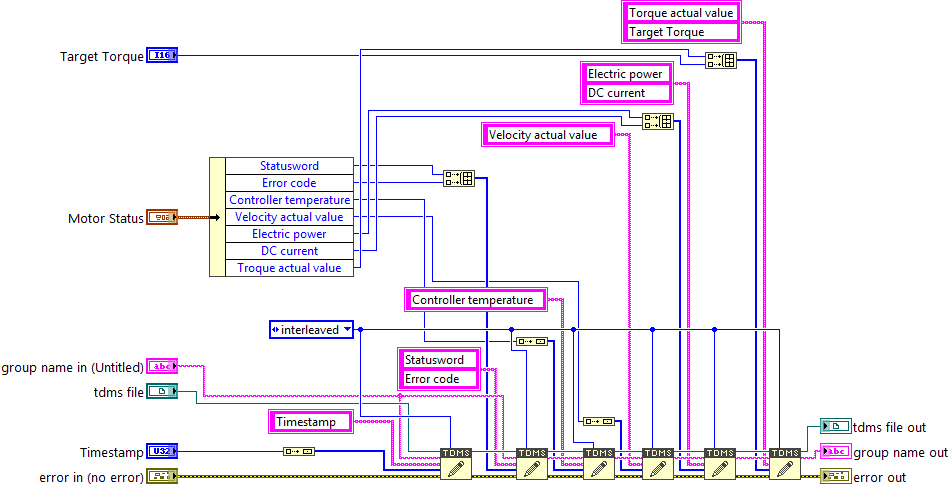
\includegraphics[width=\textwidth]{figures/Motor_to_TDMSd}
    \caption{Motor\_to\_TDMS.vi}
    \label{vi:Motor_to_TDMS}
\end{figure}